%Przykładowy plik ułatwiający złożenie projektu dyplomowego inżynierskiego.
%UWAGA: Generowany napis na stronie tytułowej o treści PROJEKT DYPLOMOWY INŻYNIERSKI został zaproponowany przeze mnie i nie jest, póki co, potwierdzony przez władze wydziału. Przed ostatecznym oddaniem tak złożonej pracy należy upewnić się jaka powinna być treść tego napisu. W momencie gdy uzyskam informację na temat treści tego napisu, dokonam niezbędnych zmian w źródłach.
\documentclass[printmode]{mgr}
%opcje klasy dokumentu mgr.cls zostały opisane w dołączonej instrukcji

%poniżej deklaracje użycia pakietów, usunąć to co jest niepotrzebne
%\usepackage{polski} %przydatne podczas składania dokumentów w j. polskim
\usepackage[polish]{babel}%alternatywnie do pakietu polski, wybrać jeden z nich
%\usepackage[OT4,plmath]{polski}
\usepackage[utf8]{inputenc} %kodowanie znaków, zależne od systemu
\usepackage[T1]{fontenc} %poprawne składanie polskich czcionek

%pakiety do grafiki
\usepackage{subfigure}
\usepackage{listings}
\usepackage{graphicx}
\usepackage{epstopdf}
\usepackage{subfigure}
\usepackage{psfrag}

\lstset{ %
language=C++,                	% choose the language of the code
basicstyle=\scriptsize,       		% the size of the fonts that are used for the code
numbers=left,                   % where to put the line-numbers
numberstyle=\footnotesize,      % the size of the fonts that are used for the line-numbers
stepnumber=2,                   % the step between two line-numbers. If it's 1 each line 
                                % will be numbered
numbersep=5pt,                  % how far the line-numbers are from the code
showspaces=false,               % show spaces adding particular underscores
showstringspaces=false,         % underline spaces within strings
showtabs=false,                 % show tabs within strings adding particular underscores
frame=single,	                % adds a frame around the code
tabsize=2,	                % sets default tabsize to 2 spaces
captionpos=b,                   % sets the caption-position to bottom
breaklines=true,                % sets automatic line breaking
breakatwhitespace=false,        % sets if automatic breaks should only happen at whitespace
title=\lstname,                 % show the filename of files included with \lstinputlisting;
                                % also try caption instead of title
escapeinside={\%*}{*)},         % if you want to add a comment within your code
morekeywords={*,...}            % if you want to add more keywords to the set
}

%pakiety dodające dużo dodatkowych poleceń matematycznych
\usepackage{amsmath}
\usepackage{amsfonts}

%pakiety wspomagające i poprawiające składanie tabel
\usepackage{supertabular}
\usepackage{array}
\usepackage{tabularx}
\usepackage{hhline}

%pakiet wypisujący na marginesie etykiety równań i rysunków zdefiniowanych przez \label{}, chcąc wygenerować finalną wersję dokumentu wystarczy usunąć poniższą linię
%\usepackage{showlabels}

%definicje własnych poleceń
\newcommand{\R}{I\!\!R} %symbol liczb rzeczywistych, działa tylko w trybie matematycznym
\newtheorem{theorem}{Twierdzenie}[section] %nowe otoczenie do składania twierdzeń

%dane do złożenia strony tytułowej
\title{Podatny manipulator planarny - budowa i sterowanie}
\engtitle{Compliant planar manipulator - design and control}
\author{Michał Kot}
\supervisor{dr inż. Janusz Jakubiak, I-6}
%\guardian{dr hab. inż. Imię Nazwisko Prof. PWr, I-6} %nie używać jeśli opiekun jest tą samą osobą co prowadzący pracę

%\date{2008} %standardowo u dołu strony tytułowej umieszczany jest bieżący rok, to polecenie pozwala wstawić dowolny rok

%poniżej jest lista kierunków i specjalności na wydziale elektroniki, należy wybrać właściwe lub dopisać jeśli nie ma odpowiednich
\field{Automatyka i Robotyka (AIR)}
\specialisation{Robotyka (ARR)}

%tutaj zaczyna się właściwa treść dokumentu
\begin{document}
\bibliographystyle{plabbrv} %tylko gdy używamy BibTeXa, ustawia polski styl bibliografii

\maketitle %polecenie generujące stronę tytułową
\tableofcontents %spis treści

%poniżej znajduje się przykładowa treść dalszej części dokumentu, zainteresowanych zachęcam do rozszyfrowania frazy "Lorem ipsum" :)

\chapter{Wstęp}
Z roku na rok rośnie liczba robotów, które są w stanie zastąpić człowieka w mniej lub bardziej skomplikowanych czynnościach. Ponadto,
coraz częściej spotyka się operacje, w których ludzie i roboty współpracują ze sobą. Wiąże się to ze zwiększonymi wymogami bezpieczeństwa, 
ponieważ człowiek ze względu na delikatną budowę jest narażony na mechaniczne uszkodzenia ciała. Jednym z rozwiązań
zapewniających bezinwazyjną pracę robota jest wykorzystanie struktury równoległej i redundantnej, co pozwala kontrolować siły, którymi
robot oddziałuje na otaczające go obiekty. W przypadku pojawienia się w przestrzeni roboczej małych i lekkich obiektów robot
jest w stanie je przesunąć używając nieznacznie większej siły, podczas gdy cięższe przeszkody prowadzą do modyfikacji
konfiguracji bądź też całej trasy manipulatora. W związku z tym pojawienie się człowieka w położeniu kolidującym z trajektorią ruchu
robota nie spowoduje znaczącego wzrostu pojawiających się sił, a co więcej wymusi generację nowej bezkolizyjnej ścieżki jeśli to będzie możliwe.

W niniejszej pracy magisterskiej podjęta zostanie próba zaprojektowania i skonstruowania takiego robota, który
będzie w stanie nieinwazyjnie koegzystować z obiektami znajdującymi się w jego otoczeniu. Struktura kinematyczna
jest kluczowym aspektem budowania bezpiecznego modelu manipulatora, w związku z tym warto przyjrzeć się kilku
cechom, które taki robot powinien posiadać.

\section{Manipulator równoległy}
Roboty o strukturach równoległych definiuje się jako roboty, w których platforma ruchoma, tzn. sprzęg efektora, jest połączona
z podstawą -- platformą więcej niż jednym łańcuchem kinematycznym, tworząc zamknięty łańcuch kinematyczny \cite{honczarenko}.
Budowa taka ma szereg istotnych zalet w stosunku do konstrukcji konwencjonalnych -- osie napędowe manipulatora
mogą być umieszczone u jego podstawie, dzięki czemu znacząco zredukowana jest masa części ruchomej. Umożliwia to precyzyjniejsze sterowanie,
a także uzyskiwanie większych przyspieszeń ze względu na zmniejszoną bezwładność. Ponadto siły zewnętrzne działające na efektor
nie są przenoszone przez szeregowy łańcuch elementów, lecz rozłożone na równoległe ramiona, co wpływa na dużą sztywność struktury układu.
Stosunek masy do sztywności układu ulega znaczącej poprawie.

Z drugiej strony wprowadzenie równoległej struktury znacząco zwiększa złożoność równań opisujących prostą i odwrotną kinematykę robota.
Ponadto, ograniczeniu ulega przestrzeń robocza, która może być dużo mniejsza niż gabaryty manipulatora. Równoległość niesie za sobą
także pojawianie się konfiguracji osobliwych, które komplikują sterowanie robotem i wymagają stosowania odpowiednich ograniczeń.
W strukturach równoległych występują też możliwe kolizje pomiędzy ramionami, a efektorem robota, co należy uwzględnić przy
definiowaniu dopuszczalnego zakresu ruchu.

Najczęściej spotyka się roboty równoległe o trzech lub nawet sześciu ramionach \cite{honczarenko}. Mimo dużej liczby napędów uzyskuje
się w nich dość niewielką liczbę stopni swobody. Ich największą zaletą jest to, że silniki i przekładnie są zamocowane
na nieruchomej podstawie (co więcej poza przestrzenią roboczą), przez co nie obciążają członów ruchomych i nie pogarszają w ten sposób
właściwości dynamicznych robota. Podobnie sytuacja wygląda w manipulatorze stworzonym w ramach tego projektu, jednakże zastosowane
zostały dwa ramiona.

\section{Manipulator redundantny} \label{sec:redundantny}
Manipulator redundantny (nadmiarowy) składa się z większej liczby przegubów niż jest ona wymagana do wykonania konkretnego zadania. 
Cecha ta zapewnia to robotowi większą zręczność, która pozwala na skuteczne omijanie osobliwości, ograniczeń przegubów czy
przeszkód pojawiających się w przestrzeni roboczej \cite{handbook}. Wpływa to korzystnie na rozmiar samej przestrzeni roboczej,
ponieważ liczba osiągalnych konfiguracji ulega zwiększeniu. Co więcej, zmniejszone są także energia i momenty w przegubach,
co wpływa na poprawę dynamicznych osiągów robota. Dla manipulatorów redundantnych komplikacji ulega zadanie odwrotnej kinematyki, ponieważ istnieje nieskończona liczba jej rozwiązań. W związku z tym definiuje się kryteria doboru konfiguracji, tak aby obliczone położenia przegubów były optymalne. 


\section{Manipulator planarny}
Planarność, jako cecha manipulatora, oznacza, że porusza się on jedynie na płaszczyźnie, a nie w przestrzeni trójwymiarowej.
Położenie efektora opisuje się za pomocą współrzędnych położenia X i Y oraz orientacji $\theta$. Takie ograniczenie znacząco redukuje 
stopień złożoności ruchu robota, a w konsekwencji równania opisujące jego ruch. Przy konstruowaniu manipulatorów
planarnych istotna jest redukcja masy ruchomych elementów, ponieważ nie posiadają one napędów redukujących wpływ siły grawitacji.

\section{Manipulator podatny}
Podatność \cite{handbook} definiowana jest jako możliwość kontroli sił, którymi robot oddziałuje
na otoczenie bez precyzyjnej znajomości środowiska, w którym się znajduje. Wykorzystanie jedynie prędkości i przyspieszeń
do sterowania ruchu manipulatora prowadzi do pojawiania się dużych sił przy kontakcie z niespodziewanymi obiektami. Pojawiające się
w tym momencie przyspieszenia prowadzą do sporych rozbieżności i błędów pozycjonowania efektora. Problem ten może być
rozwiązany poprzez wprowadzenie równoległego sterowania siłą, które umożliwia regulację wartości oddziaływania efektora
na otoczenie. Kontrolowanie siły efektora znajduje swoje zastosowanie zarówno przy zatrzymywaniu ruchu robota w kontakcie z
obiektami sztywnymi, jak i zręcznym manipulowaniu obiektami miękkimi (np. chwytanie gąbki).

Popularnym podejściem do sterowania manipulatora w kontakcie z nie w pełni znanym środowiskiem jest wykorzystanie hybrydowego
połączenia sterowania przyspieszeniem i siłą. Kontrolowanie samej siły nie zapewnia odpowiednich właściwości dynamicznych ruchu
robota, podczas gdy bez sterowanie przyspieszeniem w kontakcie z przeszkodami prowadzi do błędów wspomnianych wcześniej. 
O ile zastosowanie obu sterowań równolegle jest dość skomplikowane, stosuje się pewne uproszczenia pozwalające zdekomponować
problem na dwa części. Możliwe jest rozdzielenie stopni swobody robota na pracę w domenie sił i przyspieszeń w taki sposób,
aby nie zachodziły one na siebie. W rezultacie, można otrzymać manipulator sterujący siłą/momentem jedynie w dwóch kierunkach,
podczas gdy w pozostałych sterowanie odbywa się standardowo z wykorzystaniem przyspieszeń.


\chapter{Cele projektu} \label{ch:cele}
Celem projektu zrealizowanego w ramach niniejszej pracy magisterskiej jest zaprojektowanie i skonstruowanie planarnego, równoległego
i redundantnego manipulatora, który będzie w stanie analizować siły działające na niego z zewnątrz. Umożliwi to 
zręczne poruszanie się robota w środowisku, ponieważ każda napotkana przeszkoda spowoduje zatrzymanie go bądź też zmusi
do osiągnięcia zadanego położenia w innej konfiguracji przegubów. Dodatkową cechą, która zostanie zaimplementowana w manipulatorze
jest możliwość uczenia się ruchów zadanych manualnie przez operatora -- konkretna ścieżka może zostać zapisana na podstawie
odczytów sił działających na napędy. 

\section{Aspekt inżynierski}
Aspekt inżynierski projektu zakłada zaprojektowanie mechaniki i układu sterowania manipulatora. Jest on ściśle powiązany
z aspektem badawczym (\ref{sec:aspekt_badawczy}), ponieważ dobór parametrów układu mechanicznego musiał zostać poprzedzony
szeregiem analiz i symulacji. Trójwymiarowy model obiektu został wykonany z wykorzystaniem środowiska \texttt{Autodesk Inventor} \cite{autodesk},
które to umożliwia szybkie i wygodnie modelowanie złożonych konstrukcji mechanicznych. Co więcej, posiada on plugin
\texttt{SimMechanics Link} \cite{simmechanics_link}, umożliwiający eksport modelu do toolboxa \texttt{Simulink} środowiska 
\texttt{Matlab} \cite{mathworks}, które jest jednym z najpopularniejszych i najbardziej rozbudowanych aplikacji symulacyjnych.
W trakcie prac z wykorzystaniem Inventora skonstruowane zostały cztery podobne modele manipulatora, które ewoluowały 
w kierunku wersji docelowej. 

Projektowanie i implementacja algorytmów sterowania ..... Tu będzie dalszy tekst, gdy zacznę prace nad tym etapem.

\section{Aspekt badawczy}\label{sec:aspekt_badawczy}
Opracowanie kryteriów doboru parametrów kinematycznych manipulatora stanowiło jeden z kluczowych elementów aspektu badawczego projektu.
Proporcje długości ramion robota mają istotny wpływ na jakość i wielofunkcyjność jego pracy, w związku z czym definiuje się cały
szereg kryteriów \cite{miary_jakosci}, które różnią się pomiędzy sobą zarówno podejściem, jak i stopniem skomplikowania:
\begin{itemize}
\item ekscentryczność manipulatora, mierząca odległość położenia przegubów od ich pozycji środkowych,
\item manipulowalność manipulatora, która jest miarą wrażliwości efektora na lokalne wariacje konfiguracji,
\item współczynnik uwarunkowania, będący miarą stopnia anizotropowości konfiguracji,
\item dystorsja kinematyczna, jako miara niesztywności kinematyki,
\item objętość przestrzeni roboczej,
\item gęstość objętości kinematyki.
\end{itemize}
W teorii robotyki stosuje się także kombinacje kilku różnych kryteriów. W przypadku niniejszego projektu zastosowane zostało
kryterium mówiące o objętości przestrzeni roboczej, co w przypadku manipulatorów planarnych sprowadza się do powierzchni przestrzeni roboczej. 
Obliczenie przestrzeni z dużą dokładnością dla wielu różnych konfiguracji robota jest niemożliwe bez wykorzystania komputera. W związku
z tym konieczne okazało się napisanie programu z wykorzystaniem języka C++, który wyszukuje optymalną konfigurację parametrów manipulatora. 
Szerzej zostało to opisane w rozdziale \ref{sec:wyznaczenie_wymiarow_manipulatora}.

Istotną częścią aspektu badawczego projektu były także badania porównawcze algorytmów sterowania oraz ocena ich własności.
.....
Tu będzie dalszy tekst, gdy zacznę prace nad tym etapem.


\chapter{Pierwowzór} \label{ch:pierwowzor}
Pomysł na stworzenie planarnego manipulatora zrodził się po przeczytaniu artykułu naukowego
"Hybrid position/force control of a flexible parallel manipulator" \cite{wzor}. 
Autorzy tego artykułu podjęli się stworzenia równoległego manipulatora, którego cechą charakterystyczną
jest elastyczna końcówka umożliwiająca pomiary sił/momentów działających na efektor. 
Jak widzimy na rysunku \ref{rys:pierwowzor_zdjecie}, do pomiaru siły został wykorzystany czujnik sił/momentów
o sześciu stopniach swobody, dzięki czemu możliwe jest wykrycie każdego rodzaju deformacji elastycznej
końcówki. Zaletą takiego rozwiązania jest zdolność do analizy sił i momentów, którymi otoczenie
oddziałuje na efektor. W rezultacie, poprzez zastosowanie hybrydowego sterowania, polegającego
na jednoczesnym kontrolowaniu położenia efektora i sił na niego oddziałujących, jesteśmy w stanie zapewnić
dokładniejszą i bezpieczniejszą interakcję manipulatora z otoczeniem. Wynika to z braku dużych sił powstających
przy wykorzystaniu jedynie kontroli położenia.
\begin{figure}[tp]
\centering
  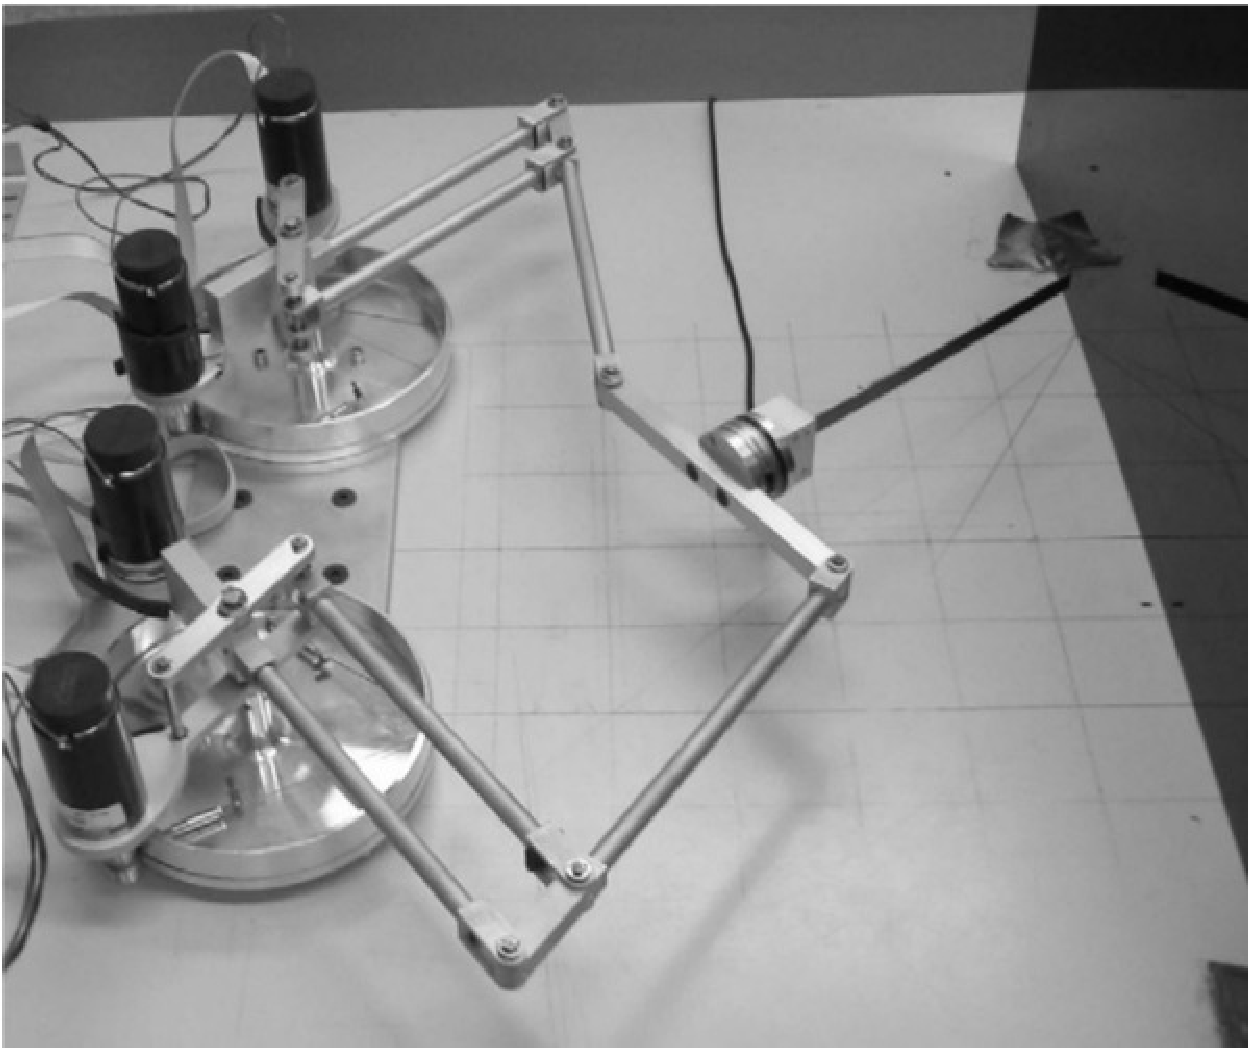
\includegraphics[width=0.6\textwidth]{grafika/pierwowzor_zdjecie}
  \caption{Pierwowzór konstruowanego manipulatora}
  \label{rys:pierwowzor_zdjecie}  
\end{figure}

\section{Różnice w stosunku do pierwowzoru}\label{sec:roznice_do_pierwowzoru}
Stworzony w ramach niniejszej pracy magisterskiej manipulator różni się jednakże w wielu aspektach od
swojego pierwowzoru. Na rysunku \ref{rys:pierwowzor_model} znajduje się model pierwowzoru, jednakże po szeregu badań i analiz 
okazało się, że konstrukcja tamtego manipulatora nie zakładała redundancji, która jest jednym z
fundamentów tego projektu. Redundancja, która umożliwia osiągnięcie jednego położenia efektora przy pomocy
wielu różnych konfiguracji manipulatora, została zapewniona poprzez wprowadzenie jednego dodatkowego przegubu
pasywnego. Co więcej, w stosunku do pierwowzoru elastyczne ramie połączone z czujnikiem sił i momentów
zostało zastąpione przez inny mechanizm, opisany dokładniej w rozdziale \ref{sec:czujniki_sily}.
Dzięki zmianom w konstrukcji manipulator stworzony w ramach tego projektu posiada większą gamę
potencjalnych zastosowań, np. możliwość uczenia się. 

\begin{figure}[tp]
\centering
  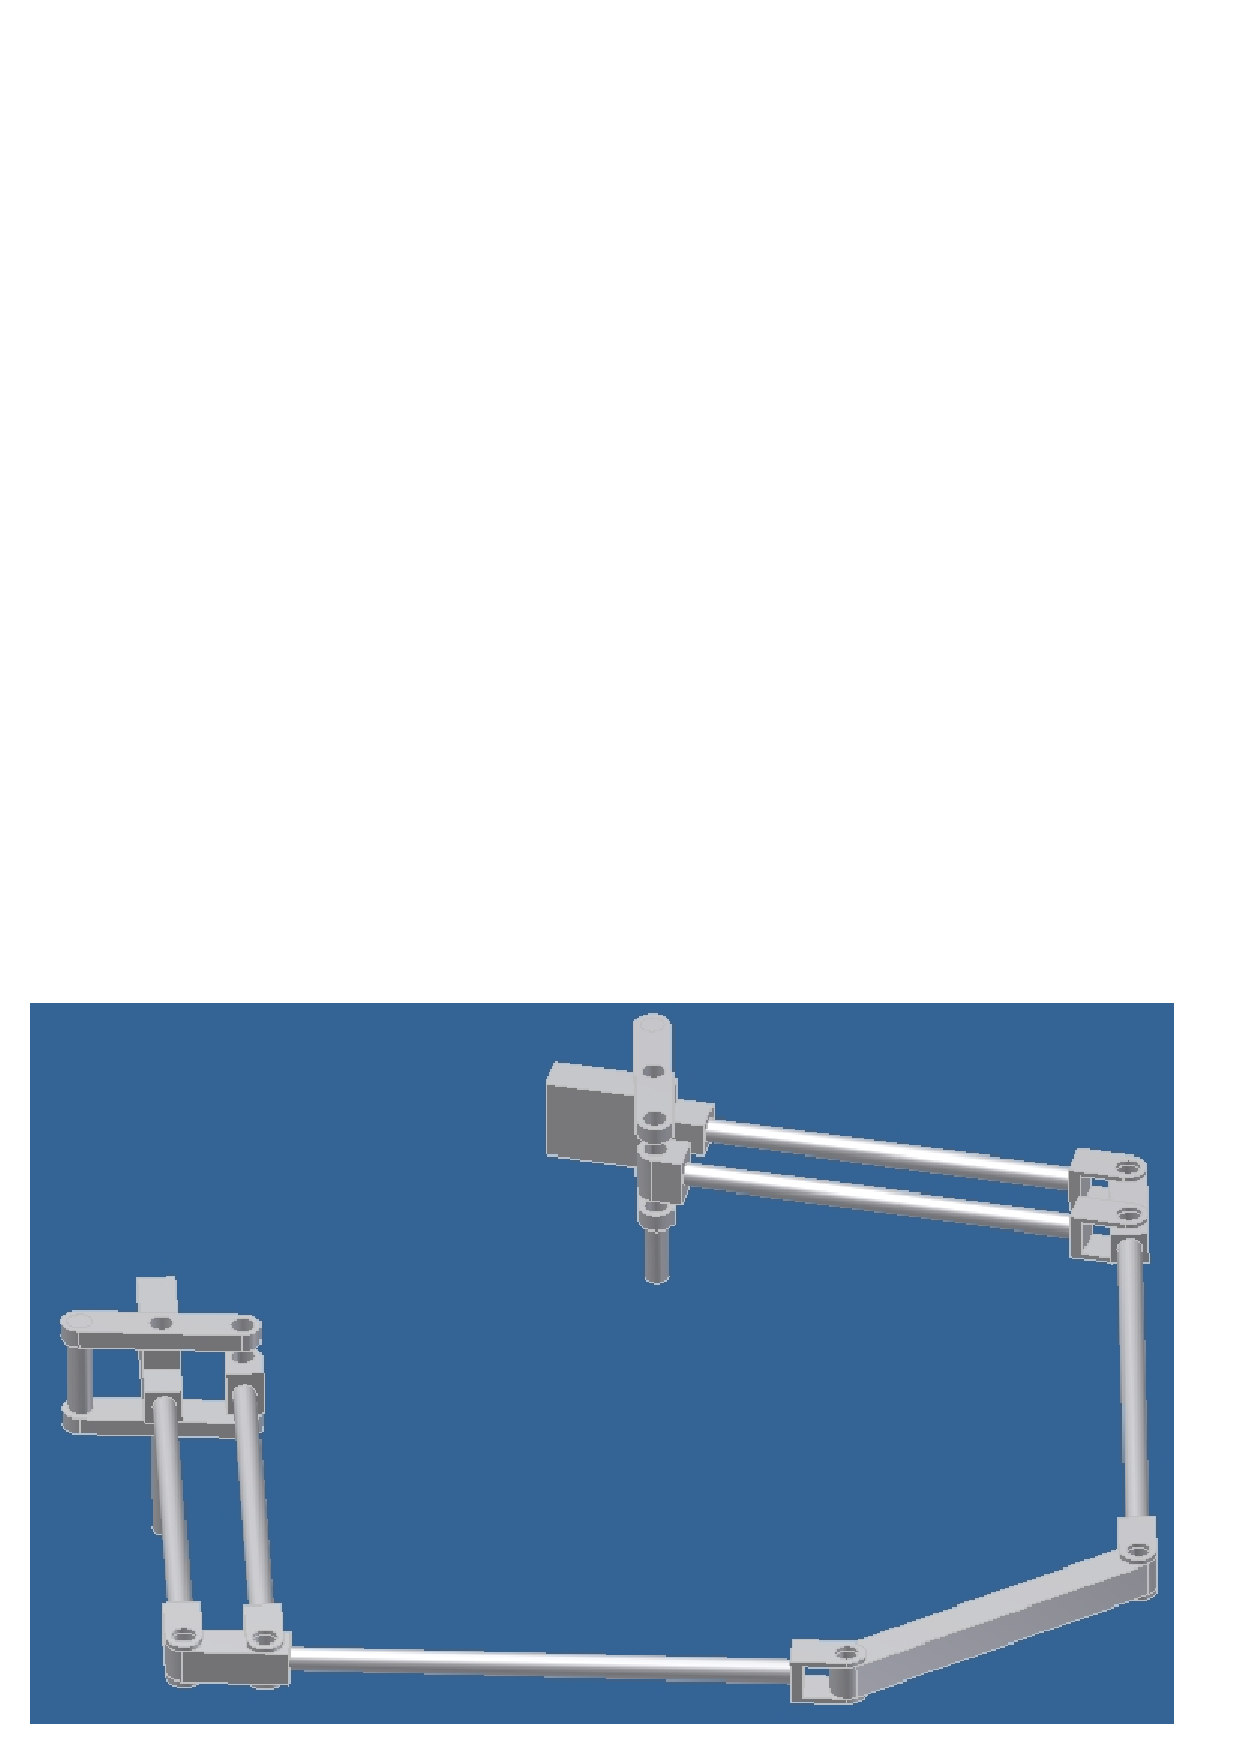
\includegraphics[width=0.6\textwidth]{grafika/pierwowzor_model}
  \caption{Model pierwowzoru konstruowanego manipulatora}
  \label{rys:pierwowzor_model}  
\end{figure}


\section{Inne projekty wykorzystujące podobne rozwiązania}
Przed przystąpieniem do projektowania manipulatora przeanalizowane zostały podobne rozwiązania, które
dostarczyły pomysłów dla realizacji projektu. Praca \cite{inne1} przedstawia konstrukcję podatnego manipulatora planarnego,
który ma możliwość operowania i interakcji z obiektami, które nie są precyzyjnie umieszczone w jego otoczeniu.
Zastosowane tam zostały innowacyjne algorytmy sterowania pozwalające kontrolować sztywność i impedancję manipulatora.
Dzięki sprężynom umieszczonym szeregowo z ramionami robot kontroluje siły oddziałujące na niego z otoczenia. 
W samej pracy znajduje się szereg badań i analiz, które przedstawiają wydajność takiego rozwiązania.

W artykule \cite{inne2} znajduje się inny algorytm sterowania podatnego manipulatora planarnego, oparty na
strategii AFC (active force control -- aktywne sterowanie siłą). Podejście to w połączeniu z regulatorem PID
w skuteczny sposób redukuje zaburzenia pozycjonowania ramion robota. Całość została przetestowana na równoległym manipulatorze typu RRR
o trzech stopniach swobody, dla którego w raporcie wyprowadzone zostały prosta i odwrotna kinematyka.

Interesujący robot o dwóch stopniach swobody znajduje się w artykule \cite{inne3}. Jest to planarny, równoległy manipulator 
wykorzystywany przy pracy z systemami półprzewodnikowymi. Ze względu na minimalizację masy poruszających się elementów
robot pozycjonowany jest z niezwykle dużą dokładnością, co jest wymagane przy pracy z półprzewodnikami. Zwiększenie precyzji
pozycjonowania efektora na płaszczyźnie XY otrzymano poprzez zastosowanie równoległej budowy robota. W raporcie tym znajduje
się także bogate porównanie z tradycyjnymi metodami sterowania, uwypuklające wady i zalety mechanizmów równoległych.

Dynamikę i sterowanie manipulatora redundantnego można znaleźć w pracy \cite{inne4}. Bazując na modelu dynamiki przedstawione
są strategie sterowania pozycją i siłą, stosowane naprzemiennie. Zdefiniowane są krytyczne kąty przegubów, przy których następuje zmiana
strategii. W raporcie tym znajdują się badania porównujące jakość pozycjonowania efektora dla redundantnej i nieredundantnej wersji manipulatora.
Na podstawie przeprowadzonych eksperymentów autorzy stwierdzają, że błędy w obu przypadkach są do siebie zbliżone. Istotnym wnioskiem jest
fakt, że wprowadzenie redundacji nie wpływa na jakość pozycjonowania, a jednocześnie zwiększa możliwości sztywność i możliwości manipulacyjne robota.

\section{Testowe modele manipulatora}
Przed pojawieniem się finalnej wersji manipulatora rozważane były różne warianty, a projekt ewoluował od pierwowzoru \ref{rys:pierwowzor_model}
do wersji finalnej \ref{rys:manipulator_docelowy_model}. Wersja oparta na pierwowzorze została odrzucona po pierwszych
testach, głównie ze względu na wady opisane w sekcji \ref{sec:roznice_do_pierwowzoru}. 
\begin{figure}[tp]
\centering
  \includegraphics[width=0.6\textwidth]{grafika/testowa_wersja_model}
  \caption{Testowy model manipulatora}
  \label{rys:testowa_wersja_model}  
\end{figure}

Model kolejnego rozpatrywanego wariantu znajduje się na rysunku \ref{rys:testowa_wersja_model}. W stosunku do pierwowzoru pojawił
się jeden dodatkowy przegub, który zapewnił redundancję manipulatora. Ponadto efektorem jest sztywna część (w pierwowzorze była elastyczna),
co całkowicie zmienia sposób sterowania i wykorzystania czujników siły. Kinematyka prosta, polegająca
na obliczaniu pozycji efektora ($x_e, y_e, \theta_e$) na podstawie położeń przegubów ($q_{a1}, q_{a2}, q_{b1}, q_{b2}$)
znajduje się w równaniach \ref{eq:testowa_kinematyka_prosta} i \ref{eq:testowa_kinematyka_prosta2}.
\begin{equation}
\begin{cases}
x_e = l_4\cos\theta_e - \sin(\arctan(\frac{y_a-y_b}{x_a-x_b}))\sqrt{l_3^2-(\frac{1}{2}\sqrt{(x_a-x_b)^2+(y_a-y_b)^2})^2} + \frac{1}{2}(x_a+x_b),\\
y_e = l_4\sin\theta_e + \cos(\arctan(\frac{y_a-y_b}{x_a-x_b}))\sqrt{l_3^2-(\frac{1}{2}\sqrt{(x_a-x_b)^2+(y_a-y_b)^2})^2} + \frac{1}{2}(y_a+y_b),\\
\theta_e = \frac{3}{2}\pi - \beta - \arctan(\frac{- \sin(\arctan(\frac{y_a-y_b}{x_a-x_b}))\sqrt{l_3^2-(\frac{1}{2}\sqrt{(x_a-x_b)^2+(y_a-y_b)^2})^2} + \frac{1}{2}(x_a-x_b)}{\cos(\arctan(\frac{y_a-y_b}{x_a-x_b}))\sqrt{l_3^2-(\frac{1}{2}\sqrt{(x_a-x_b)^2+(y_a-y_b)^2})^2} + \frac{1}{2}(y_a-y_b)}) ,
\end{cases}
\label{eq:testowa_kinematyka_prosta}
\end{equation}
gdzie
\begin{equation}
\begin{cases}
x_a = L + l_1\cos q_{a1} + l_2 \cos(q_{a1}+q_{a2}),\\
x_b = -L + l_1\cos q_{b1} + l_2 \cos(q_{b1}+q_{b2}),\\
y_a = l_1\sin q_{a1} + l_2 \sin(q_{a1}+q_{a2}),\\
y_b = l_1\sin q_{b1} + l_2 \sin(q_{b1}+q_{b2}),\\
\beta = \frac{2}{3}\pi.
\end{cases}
\label{eq:testowa_kinematyka_prosta2}
\end{equation}

Stała wartość $\beta$ oznacza kąt pomiędzy ostatnim ogniwem lewego ramienia, a ogniwem efektora. W modelu na rysunku \ref{rys:testowa_wersja_model},
a także we wszystkich symulacjach wynosi on 120 stopni. Punkty $(x_a, y_a)$ oraz $(x_b, y_b)$ reprezentują zakończenia pierwszych
dwóch ramion (odpowiednio prawego i lewego), tworzących dwuwahadło.

Zadaniem kinematyki odwrotnej jest wyznaczenie położeń przegubów ($q_{a1}, q_{a2}, q_{b1}, q_{b2}$) przy znanej pozycji efektora
($x_e, y_e, \theta_e$). Równania \ref{eq:testowa_kinematyka_odwrotna} i \ref{eq:testowa_kinematyka_odwrotna2} zawierają te przekształcenia.

\begin{equation}
\begin{cases}
q_{a1} = \arctan(\frac{y_a}{x_a-L})-\arccos(\frac{l_1^2-l_2^2+(x_a-L)^2+y_a^2}{2l_1\sqrt{(x_a-L)^2+y_a^2}}),\\
q_{a2} = \pi - \arccos(\frac{l_1^2+l_2^2-(x_a-L)^2-y_a^2}{2l_1l_2}),\\
q_{b1} = \arctan(\frac{y_b}{x_b+L}) + \arccos(\frac{l_1^2-l_2^2+(x_b+L)^2+y_b^2}{2l_1\sqrt{(x_b+L)^2+y_b^2}}),\\
q_{b2} = -\pi + \arccos(\frac{l_1^2+l_2^2-(x_b+L)^2-y_b^2}{2l_1l_2}),
\end{cases}
\label{eq:testowa_kinematyka_odwrotna}
\end{equation}
gdzie
\begin{equation}
\begin{cases}
x_a = x_e + l_3\cos(\gamma - \theta_e) - l_4\cos(\theta_e),\\
x_b = x_e - l_3\sin(\frac{3}{2}\pi - \beta - \theta_e) - l_4\cos(\theta_e),\\
y_a = y_e - l_3\sin(\gamma - \theta_e) - l_4\sin(\theta_e),\\
y_b = y_e - l_3\cos(\frac{3}{2}\pi - \beta - \theta_e) - l_4\sin(\theta_e),\\
\beta = \frac{2}{3}\pi.
\end{cases}
\label{eq:testowa_kinematyka_odwrotna2}
\end{equation}

Parametr $\gamma$ opisuje kąt pomiędzy ostatnim ogniwem prawego ramienia, a ogniwem efektora. Ze względu na redundantny charakter manipulatora
zadanie odwrotnej kinematyki posiada nieskończoną liczbę rozwiązań. W związku z tym konieczne jest wprowadzenie dodatkowego parametru.
Kąt $\gamma$ podlega optymalizacji w trakcie procesu liczenia odwrotnej kinematyki, gdyż miał on służyć do kontrolowania równomierności
rozkładu sił działających na efektor na obydwa ramiona. Ze względu na pominięcie analizy sił dla testowej wersji manipulatora, można
przyjąć go jako wartość stałą.

Dla takiego manipulatora zostały przeprowadzone badania wielkości jego przestrzeni roboczej, jej kształtu i wpływu na rozmiar robota.
Znajdują się one w rozdziale \ref{sec:wymiary_probnej_wersji}. 
Sztywne połączenie pomiędzy efektorem, a jednym z ramion sprawia, że manipulator nie jest symetryczny względem ramion. Jest to bardzo
istotna i pożądana cecha, ponieważ zapewnia ona równomierny rozkład sił działających na efektor w obu ramionach manipulatora
(jego przegubach i silnikach). Symetryczny rozkład sił umożliwia precyzyjniejszy ich pomiar, co jest jednym z założeń projektu. 
W związku z tym ten wariant projektu został odrzucony, a w kolejnej wersji manipulator został wzbogacony o opisywaną symetrię. 
Ponadto wyeliminowanie wspomnianego sztywnego połączenia zwiększyło powierzchnię jego przestrzeni roboczej, co bezpośrednio przełożyło
się na poprawę możliwości manipulacyjnych.


\chapter{Struktura manipulatora docelowego}
Na rysunku \ref{rys:docelowy_model} znajduje się stworzony w programie \texttt{Autodesk Inventor} model
ostatecznej wersji manipulatora. Jego struktura odpowiada strukturze robota fizycznie skonstruowanego, z dokładnością
do poszczególnych części, które zostały użyte do realizacji poszczególnych elementów. Właściwości i parametry mechaniczne
konstrukcji zostaną opisane w rozdziale \ref{sec:fizyczna_realizacja} przedstawiającym fizyczną realizację manipulatora.
W tym rozdziale nacisk zostanie położony na kinematyczny aspekt budowy robota.
\begin{figure}[tp]
\centering
  \includegraphics[width=0.6\textwidth]{grafika/docelowy_model}
  \caption{Model konstruowanego manipulatora}
  \label{rys:docelowy_model}  
\end{figure}

\section{Konstrukcja manipulatora}
Konstrukcja manipulatora rozpoczyna się od czterech napędów, umieszczonych po lewej stronie na rysunku \ref{rys:docelowy_model}.
Wszystkie pozostałe przeguby są nienapędzane (pasywne). Każdym z dwóch ramion sterują dwa silniki. 
Mechanizm równoległy umieszczony na początku każdego z ramion
pozwala uzyskać możliwość manipulowania kolejnym ogniwem bez wprowadzania dodatkowego napędu, dzięki czemu
zmniejszona jest masa i bezwładność poruszającego się ramienia.
Zastosowane na końcu połączenie belki efektora z każdym z ramion w dwóch miejscach zapewnia symetryczne rozłożenie
sił działających na efektor względem obu ramion. Zastosowanie mechanizmu przesuwnego pozwala
na swobodny ruch manipulatora, przy zachowaniu równej odległości pomiędzy belką efektora i ramionami.

\section{Konfiguracje niedozwolone}\label{sec:konfiguracje_niedozwolone}
Równoległa struktura manipulatora niesie za sobą szereg ograniczeń na konfiguracje przegubów, ponieważ
istnieją potencjalne, wzajemne kolizje ramion, a także ramion i efektora. Konieczne jest wprowadzenie odpowiednich restrykcji
na zakresy kątów napędów w celu uniknięcia uszkodzeń mechanicznych robota. Mechanizm
łączący dwa silniki definiuje ograniczenie ich obrotu ze względu możliwą kolizję dwóch równoległych ogniw. 
Ponadto uszkodzenia mogą pojawić się w konfiguracjach skrajnych, w których to jedno bądź oba ramiona są mocno
skierowane ku sobie. Mogłoby to doprowadzić do zetknięcia się efektora z ramieniem bądź też ramion pomiędzy sobą.
Jednym ze sposobów zarządzania ograniczeniami jest zapewnienie wypukłości zamkniętego łańcucha manipulatora, 
które poza wyeliminowaniem potencjalnych kolizji, zapewni także również prawidłowy rozkład sił.
Konkretne ograniczenia na wartości kątów zostaną szerzej opisane w części dotyczącej implementacji, 
znajdującej się w rozdziale \ref{sec:ograniczenia_katow}.


\section{Kinematyka manipulatora}
Efektorem (chwytakiem) nazywa się zakończenie konstrukcji manipulatora, które często posiada możliwość wymiany bądź modyfikacji. 
Dzięki temu jeden robot może sekwencyjnie wykonywać kilka różniących się od siebie operacji. Pod pojęciem kinematyki kryje się
funkcja odwzorowująca przestrzeń stanu Q w orientację i położenie efektora $E_e$ \cite{podstawy_robotyki}.
Znajomość kinematyki umożliwia manipulowanie robotem, ponieważ algorytm sterowania
jest w stanie obliczyć jego aktualną konfigurację i przewidzieć zmiany, które nastąpią po aktualizacji pozycji napędów.

\subsection{Prosta kinematyka manipulatora}\label{sec:prosta_kinematyka}
Kinematyka prosta jest to przekształcenie geometryczne,
które pozwala wyznaczyć położenie i orientację efektora w przestrzeni roboczej w oparciu o położenia przegubów manipulatora.
Ze względu na planarność konstruowanego manipulatora wyznaczenie kinematyki sprowadza się do obliczenia położeń $x_e$ i $y_e$ oraz
orientacji $\theta_e$, gdyż
ruch robota odbywa się na płaszczyźnie i wartość współrzędnej Z (prostopadłej do płaszczyzny XY) jest stała.

Prostą kinematykę zaprojektowanego manipulatora zawiera równanie \ref{eq:prosta_kinematyka}.
\begin{equation}
\begin{cases}
x = ,\\
y = ,\\
\theta = .
\end{cases}
\label{eq:prosta_kinematyka}
\end{equation}

\subsection{Odwrotna kinematyka manipulatora}
Odwrotna kinematyka służy do wyznaczania wartości kątów w napędach robota ($q_1, q_2, q_3, q_4$) na podstawie informacji o 
położeniu i orientacji efektora. Jest to zadanie bardziej złożone niż kinematyka prosta, które w skrajnych przypadkach
może nie mieć rozwiązania (w momencie, gdy zadane położenie efektora jest nieosiągalne bez naruszenia ograniczeń). 
Ponadto, nawet jeśli istnieje rozwiązanie odwrotnej kinematyki, konfiguracja może być mimo wszystko nieosiągalna dla manipulatora
-- konfiguracje pośrednie, teoretycznie umożliwiające dotarcie do niej mogą naruszać zadane ograniczenia.

Redundantna struktura robota dodatkowo komplikuje zadanie odwrotnej kinematyki, ponieważ z definicji \ref{sec:redundantny}
manipulator redundantny może osiągnąć konfigurację na nieskończenie wiele sposobów. Implikuje to nieskończoną
liczbę rozwiązań zadania odwrotnej kinematyki. W związku z tym wprowadza się dodatkowy parametr (kryterium), które
wykorzystuje się do optymalizacji konfiguracji wynikowej. W tym przypadku stosuje się lokalne miary jakości, które są szczególnymi
przypadkami kryteriów przedstawionych w rozdziale \ref{sec:aspekt_badawczy}. 

Tutaj powinno być coś o konkretnym kryterium, ale jeszcze muszę to przeanalizować i wybrać najlepsze.

\begin{equation}
\begin{cases}
q_1 = ,\\
q_2 = ,\\
q_3 = ,\\
q_4 = .
\end{cases}
\label{eq:odwrotna_kinematyka}
\end{equation}

\section{Dynamika manipulatora}
Sterowanie robotem najczęściej odbywa się z wykorzystaniem modelu dynamiki. Ciała sztywne stanowiące ogniwa
manipulatora wzbogacone zostają (w stosunku do modelu kinematyki) o rozmiary geometryczne, masę i bezwładność \cite{podstawy_robotyki}.
Sterowanie oparte na modelu dynamiki lepiej sprawdza się przy precyzyjnym śledzeniu zadanej trajektorii, w szczególności
w przypadku rygorystycznych ograniczeń nakładanych na prędkości i przyspieszenia w ruchu robota. 

Ze względu na przyjętą skomplikowaną strukturę manipulatora model dynamiki w niniejszym projekcie zostanie pominięty. Zadania stawiane
przed robotem nie wymagają precyzyjnego zadawania prędkości i przyspieszeń, a zamknięty, równoległy łańcuch kinematyczny
zapewnia odpowiednią sztywność. Ponadto, redundancja i podatność robota zapewnia odpowiednią reakcję na błędy i niedokładności
przy pozycjonowaniu ogniw i efektora.


\chapter{Wyznaczenie wymiarów manipulatora}\label{sec:wyznaczenie_wymiarow_manipulatora}
Po zdefiniowaniu modelu robota w postaci równań kinematyki można przejść do projektowania
jego fizycznej konstrukcji. Pierwszym etapem tego procesu jest określenie żądanych gabarytów
robota. Istnieje kilka podejść do tego zadania \ref{sec:aspekt_badawczy}, jednakże w przypadku tej pracy została
wykorzystana analiza stosunku wielkości przestrzeni roboczej do rozmiarów poszczególnych
elementów manipulatora.

\section{Obliczenie przestrzeni roboczej manipulatora}
W celu obliczenia przestrzeni roboczej manipulatora stworzony został oddzielny program w języku C++, 
który realizował to zadanie. Składał się on przede wszystkim z klasy symulującej obiekt manipulatora, 
w której zaimplementowane zostały metody liczenia zarówno prostej jak i odwrotnej kinematyki dla
konkretnej instancji robota. Na ich podstawie wyznaczana jest przestrzeń robocza. Wyniki obliczeń
z wykorzystaniem jednej i drugiej metody zapisywane są do tej samej postaci, co pozwala na ich porównanie.

Postać ta zakłada stworzenie odpowiednio dużej siatki w przestrzeni (większej niż
przestrzeń robocza manipulatora) o określonych i równych rozmiarach pojedynczych komórek
wypełnionych zerami. Następnie wypełniamy wartościami jeden wszystkie te komórki, które są dla
poprzez efektor osiągalne dla badanego manipulatora. 

\subsection{Przestrzeń robocza na bazie prostej kinematyki}
Prosta kinematyka manipulatora zaimplementowana analogicznie do obliczeń z rozdziału \ref{prosta_kinematyka},
tutaj jest już liczona dla konkretnych wartości parametrów manipulatora. 
W celu wyznaczenia przestrzeni roboczej rozpatrzone zostały wszystkie możliwe konfiguracje
kątów przegubów manipulatora, z dokładnością do zadanego kroku i z wyłączeniem konfiguracji
niedozwolonych (opisanych szerzej w rozdziale \ref{sec:konfiguracje_niedozwolone}).
Rezultatem wyznaczenia prostej kinematyki jest położenie XY, dla którego odpowiadająca komórka
siatki przestrzeni (ta, w której efektor w zadanej konfiguracji się znajduje)
zostaje wypełniona jedynką. 

\subsection{Przestrzeń robocza na bazie odwrotnej kinematyki}
W przypadku odwrotnej kinematyki stosujemy odwrotne podejście do problemu wyznaczania przestrzeni roboczej. 
Tym razem zadanie sprowadza się do przejrzenia wszystkich komórek siatki przestrzeni i oznaczeniu
jedynką tych, dla których możliwe jest wyznaczenie konfiguracji manipulatora, w której efektor
znajduje się w aktualnej komórce. W związku z tym funkcja wyznaczająca odwrotną kinematyką
dla zadanego położenia zwraca wartość \emph{true/false} w zależności od tego czy operacja
się powiodła. 

\subsection{Obwiednia przestrzeni roboczej}
Kolejnym etapem liczenia powierzchni jest wyznaczenie obwiedni przestrzeni roboczej na podstawie
siatki wypełnionej z wykorzystaniem metod kinematyki. W tym celu został zaimplementowany algorytm, 
który dla zadanej siatki tworzy jej kopię zawierającą jedynie obrys przestrzeni. Co warto dodać,
dla efektywności obliczeń nie przeszukuje on całej siatki, a jedynie inteligentnie porusza się
po krawędziach przestrzeni roboczej (zakładamy, że jest ona wypukła). 

Dodatkowo w algorytmie została zaimplementowana możliwość zapisania wygenerowanego obrysu do pliku. 
Odbywa się to poprzez przeliczenie odpowiednich komórek siatki na wartości X i Y co umożliwia
późniejsze narysowanie przestrzeni. Przykład takiej obwiedni, wygenerowany z pomocą programu gnuplot
został przedstawiony na rysunku \ref{rys:przestrzen_robocza}. 

\subsection{Wyznaczanie powierzchni przestrzeni roboczej}
Na podstawie obwiedni przestrzeni roboczej jesteśmy w stanie obliczyć jej powierzchnię. 
Ze względu na ograniczenia numeryczne przyjęte wcześniej będzie to jedynie jej aproksymacja. 
Dla każdej kolumny obliczamy liczbę komórek siatki pomiędzy wystąpieniem pierwszej i drugiej jedynki
(górna i dolna krawędź obrysu), a następnie sumujemy wszystkie te wartości otrzymując powierzchnię przestrzeni
roboczej. Dokładność otrzymanej w ten sposób powierzchni zależy w dużym stopniu od zdefiniowanej
ziarnistości siatki. 

\section{Wyznaczenie wymiarów manipulatora na podstawie przestrzeni roboczej}
Posiadając możliwość obliczenia rozmiaru przestrzeni roboczej pojedynczej instancji 
manipulatora jesteśmy w stanie porównać je i wybrać tą, która zapewni nam najlepsze
warunki pracy. W tym celu definiujemy konkretną wartość jako sumę ramion (sama wartość nie jest istotna, gdyż
interesuje nas wzajemny stosunek długości ramion). Następnie zmieniamy długość każdego z ogniw z odpowiednim krokiem
i obliczamy rozmiar przestrzeni roboczej, zarówno prostą jak i odwrotną kinematyką. Oczywiście interesują nas tylko te
konfiguracje, w których suma długości ramion nie przekracza zadanej sumy. Spośród wszystkich wygenerowanych kombinacji wybieramy tą,
która maksymalizuje rozmiar przestrzeni roboczej. Dla zdefiniowanych ogniw należy wyznaczyć także optymalne rozstawienie
początków każdego z ramion (silników). Operację tą wykonujemy dla konkretnych długości ogniw, które z kolei musimy liczyć dla 
konkretnego rozstawienia -- zadania te są komplementarne.

\subsection{Wyznaczenie wymiarów próbnej wersji manipulatora}\label{sec:wymiary_probnej_wersji}
Przed przystąpieniem do wyznaczania konfiguracji docelowego manipulatora proces optymalizacji został przeprowadzony dla wersji próbnej,
opisanej w rozdziale \ref{rys:probna_wersja}. W tym przypadku dokładność wyniku nie była najistotniejsza, w związku z czym
wszystkie długości iterowano z krokiem 10, przy czym ich suma powinna wynosić 100. 
Po zaimplementowaniu prostej i odwrotnej kinematyki na początku wyznaczono optymalne
konfiguracje dla kilku przykładowych wartości L, będących połową odległości pomiędzy początkami ramion manipulatora:
\begin{itemize}
\item kinematyka prosta:
\begin{itemize}
\item L=0: l1=40, l2=20, l3=40, l4=0,
\item L=10: l1=30, l2=30, l3=40, l4=0,
\item L=20: l1=20, l2=40, l3=40, l4=0,
\item L=30: l1=20, l2=30, l3=50, l4=0,
\item L=40: l1=20, l2=30, l3=50, l4=0,
\end{itemize}
\item kinematyka odwrotna:
\begin{itemize}
\item L=0: l1=30, l2=40, l3=30, l4=0,
\item L=10: l1=30, l2=40, l3=30, l4=0,
\item L=20: l1=30, l2=30, l3=40, l4=0,
\item L=30: l1=30, l2=20, l3=50, l4=0,
\item L=40: l1=20, l2=30, l3=50, l4=0,
\end{itemize}
\end{itemize}
Warto wspomnieć, że parametry l1-l4 były iterowane na przedziale od 0 do 50. Jak widzimy, dla tej wersji manipulatora ostatnie z ramion
najmniej wpływa na wielkość przestrzeni roboczej, w związku z czym algorytm starał się je eliminować (dzięki temu inne ramiona mogły by dłuższe).
Przy oddalaniu początków ramion od siebie wzrasta znaczenie trzeciego ramienia, podczas gdy maleje pierwszego. Różnice pomiędzy prostą
i odwrotną kinematyką wynikają głównie z różnych metodologii liczenia, jednakże warto rozważyć i jedną i drugą opcję w celu zebrania
większej ilości obserwacji. Posiadając kilka wybranych konfiguracji manipulatora możemy teraz dokładniej już (z krokiem 1) znaleźć
najlepszą dla nich odległość L. Wyniki zostały zaprezentowane na wykresach, rysunek \ref{rys:probna_wersja_prosta_kin} prosta kinematyka
i rysunek \ref{rys:probna_wersja_odwrotna_kin}. Jak można się było spodziewać, w obu przypadkach największa przestrzeń robocza jest
osiągana dla małych wartości L. Jednakże jest to sprzeczne z wymaganiem dotyczącym rozłożenia sił działających na efektor na
poszczególne napędy -- zależy nam, aby ramiona były w pewnej odległości od siebie. W związku z tym konieczne jest wypracowanie konsensusu.
Wszystkie konfiguracje długości zwracają stosunkowo dość duże przestrzenie robocze dla parametru L znajdującego się w przedziale (10,20).
Jeżeli to byłaby ostateczna wersja manipulatora, jako kompromis wartość z tego przedziału zostałaby wybrana.

\begin{figure}[tp]
  \setlength{\unitlength}{1.0cm}
  \centering
	\subfigure[L=0: l1=40, l2=20, l3=40, l4=0]{
	  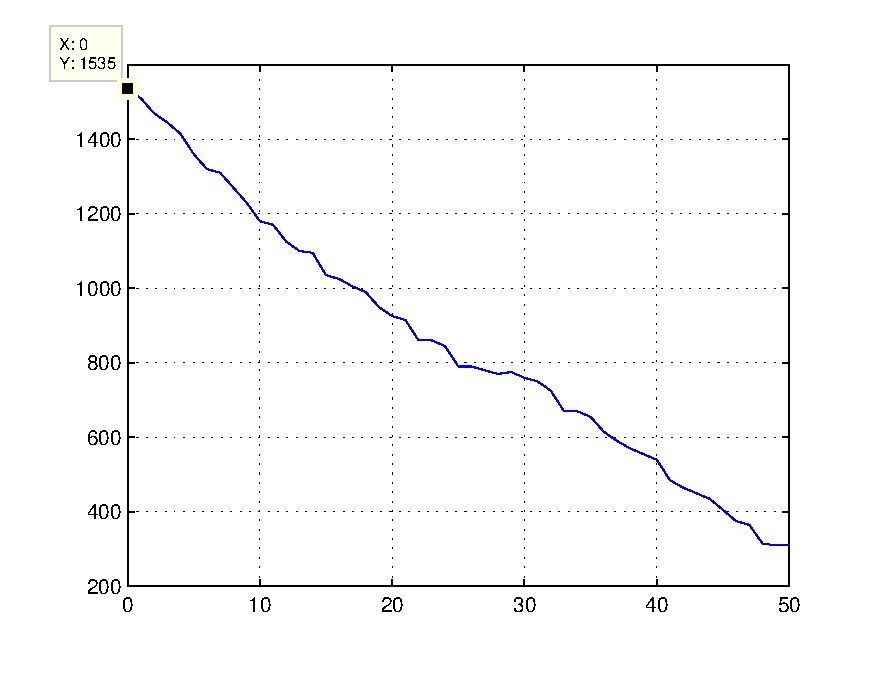
\includegraphics[width=0.4\textwidth]{grafika/probna/Forward/L=0}
	}
	\subfigure[L=10: l1=30, l2=30, l3=40, l4=0]{
	  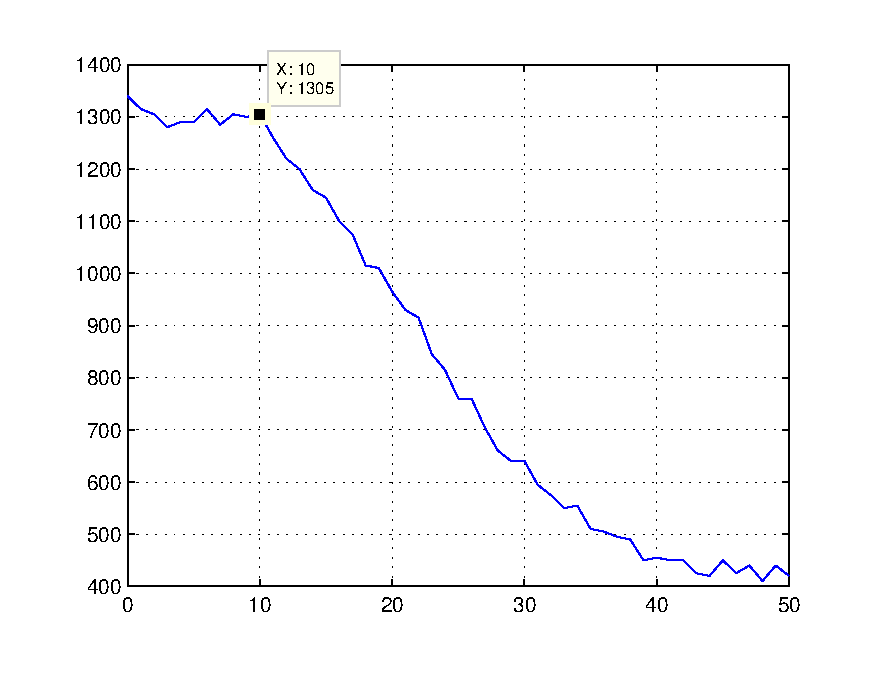
\includegraphics[width=0.4\textwidth]{grafika/probna/Forward/L=10}
	} \\
	\subfigure[L=20: l1=20, l2=40, l3=40, l4=0]{
	  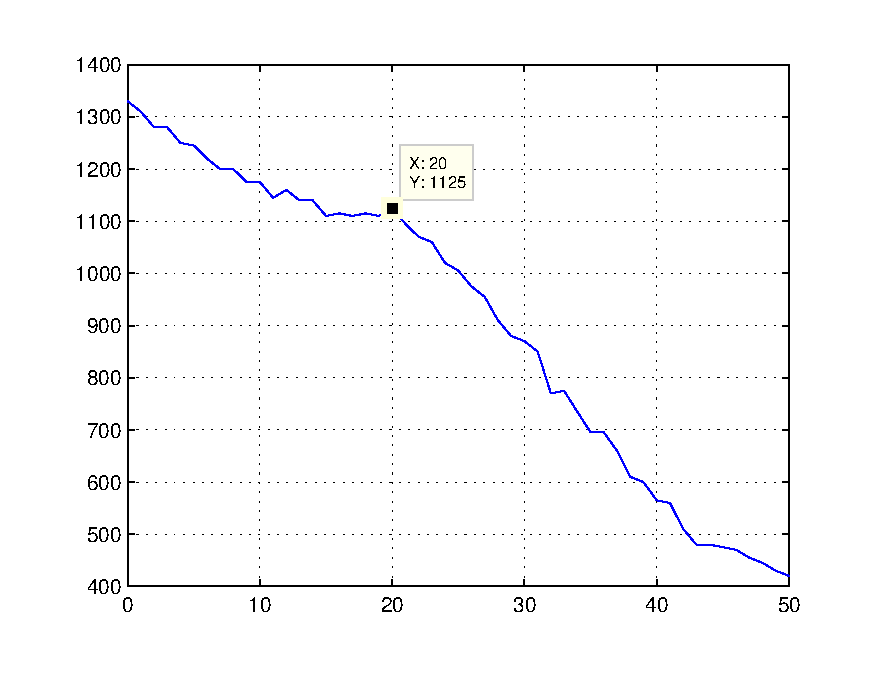
\includegraphics[width=0.4\textwidth]{grafika/probna/Forward/L=20}
	}
	\subfigure[L=30: l1=20, l2=30, l3=50, l4=0]{
	  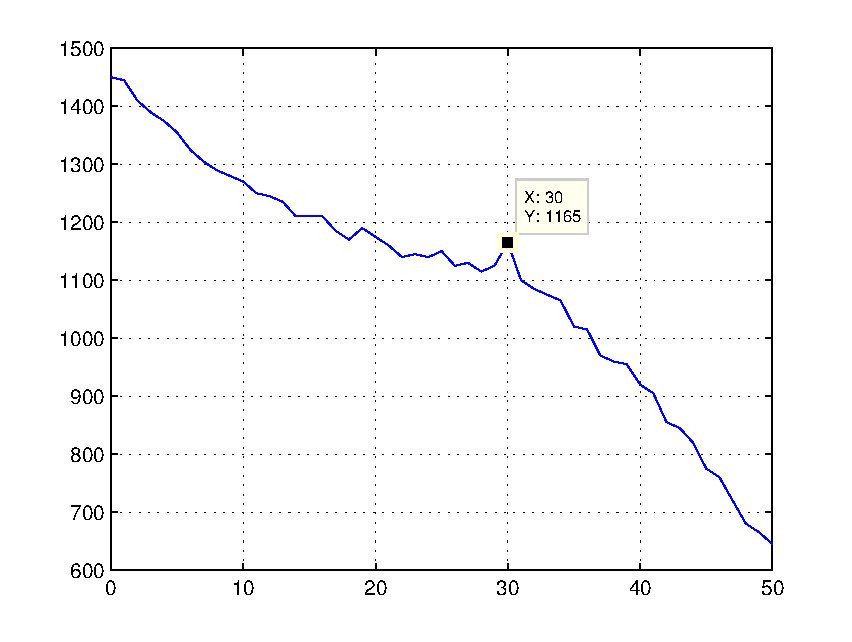
\includegraphics[width=0.4\textwidth]{grafika/probna/Forward/L=30}
	} \\
	\subfigure[L=40: l1=20, l2=30, l3=50, l4=0]{
	  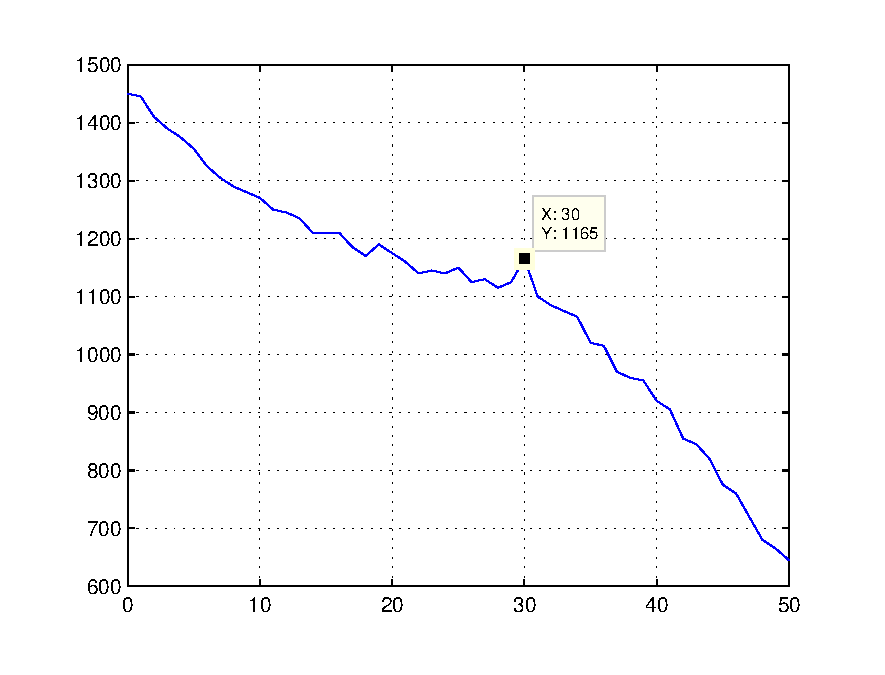
\includegraphics[width=0.4\textwidth]{grafika/probna/Forward/L=40}
	}
  \label{rys:probna_wersja_prosta_kin}  
  \caption{Powierzchnia przestrzeni roboczej w zależności od odległości początków pierwszych ramion 
  manipulatora przy wykorzystaniu prostej kinematyki}

\end{figure}

\begin{figure}[tp]
  \setlength{\unitlength}{1.0cm}
  \centering
	\subfigure[L=0: l1=30, l2=40, l3=30, l4=0]{
	  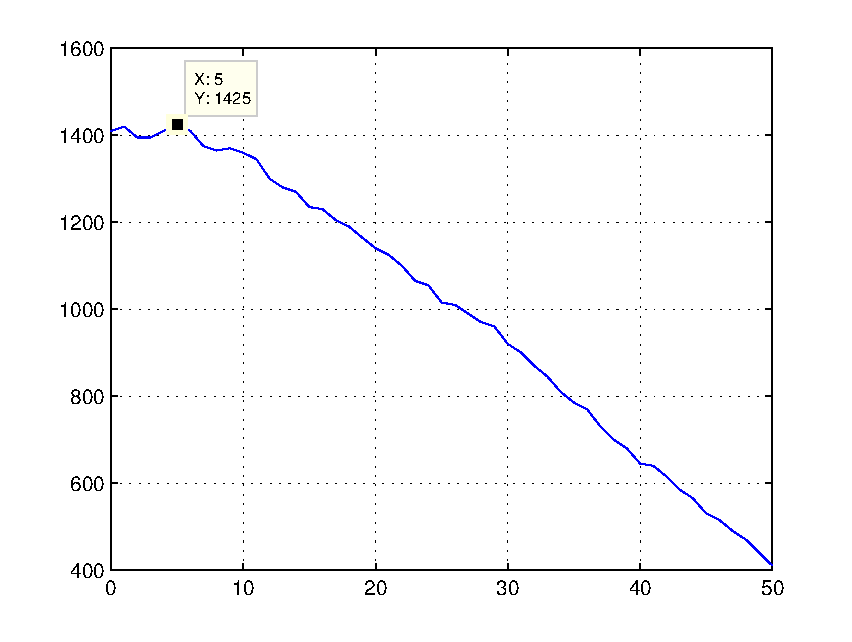
\includegraphics[width=0.4\textwidth]{grafika/probna/Inverse/L=0_inv}
	}
	\subfigure[L=10: l1=30, l2=40, l3=30, l4=0]{
	  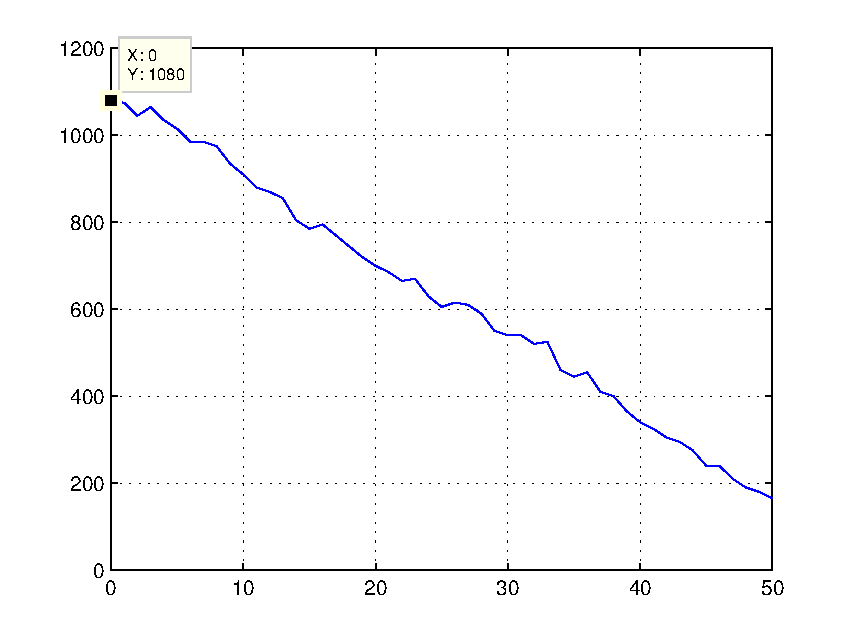
\includegraphics[width=0.4\textwidth]{grafika/probna/Inverse/L=10_inv}
	} \\
	\subfigure[L=20: l1=30, l2=30, l3=40, l4=0]{
	  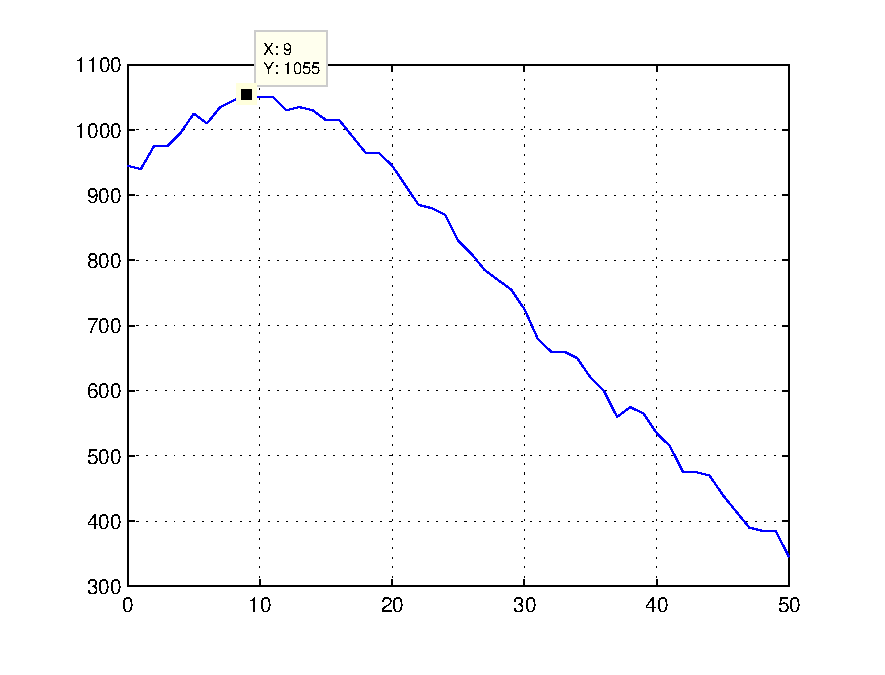
\includegraphics[width=0.4\textwidth]{grafika/probna/Inverse/L=20_inv}
	}
	\subfigure[L=30: l1=30, l2=20, l3=50, l4=0]{
	  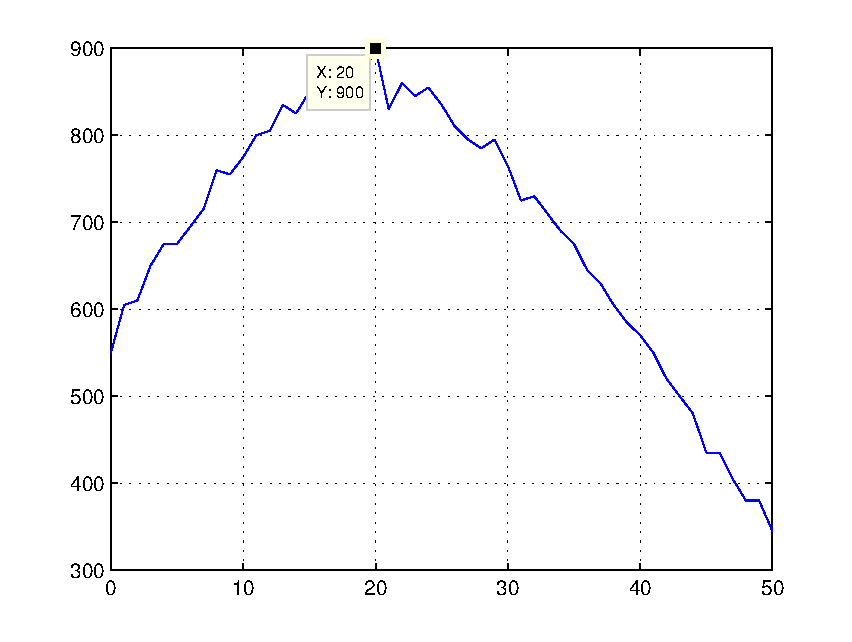
\includegraphics[width=0.4\textwidth]{grafika/probna/Inverse/L=30_inv}
	} \\
	\subfigure[L=40: l1=20, l2=30, l3=50, l4=0]{
	  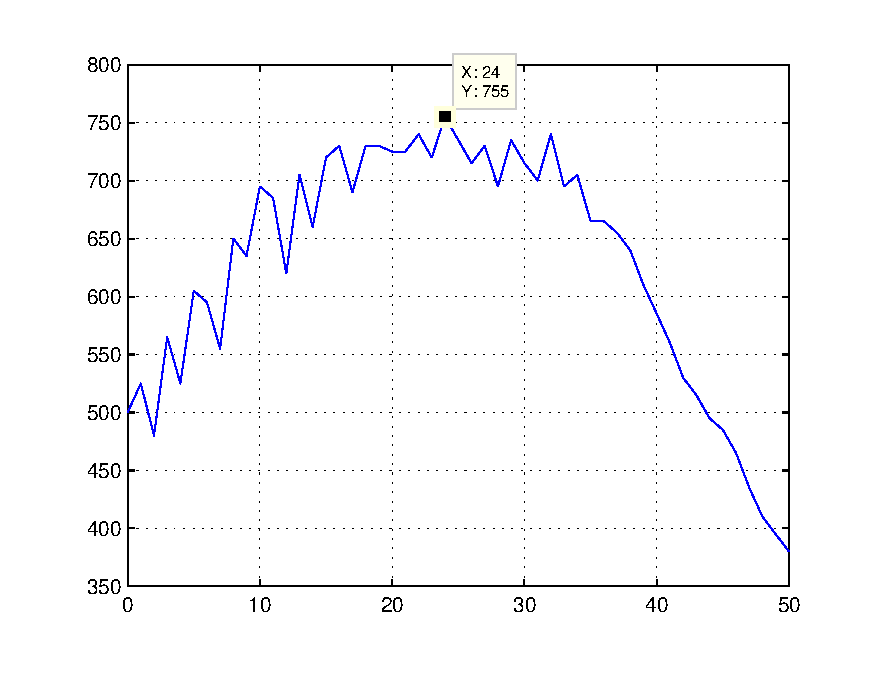
\includegraphics[width=0.4\textwidth]{grafika/probna/Inverse/L=40_inv}
	}
  \label{rys:probna_wersja_odwrotna_kin}  
  \caption{Powierzchnia przestrzeni roboczej w zależności od odległości początków pierwszych ramion 
  manipulatora przy wykorzystaniu odwrotnej}

\end{figure}

\subsection{Wyznaczenie wymiarów ostatecznej wersji manipulatora}


\chapter{Pomiar siły}
Podatność manipulatora zakłada precyzyjny pomiar sił, którymi oddziałuje on na swoje otoczenie. Rozpoznawanie
zarówno wartości, jak i kierunków sił jest zadaniem złożonym i wymaga zastosowania dużej liczby czujników, które
będą w stanie współpracować ze sobą i wzajemnie się uzupełniać. Najbardziej interesujące z punktu widzenia możliwych zastosowań
są wektory sił działających na efektor manipulatora. Z drugiej strony umieszczanie czujników na efektorze robota nie jest dobrym pomysłem,
ponieważ jest on najbardziej narażony na kontakt fizyczny, co mogłoby prowadzić do uszkodzeń mechanicznych czujników. Ponadto
prowadzenie przewodów w pobliże efektora mogłoby niekorzystnie na jego zdolności manipulacyjne, a także ze względu na odległość zwiększyć
szum pomiaru. W związku z tym do analizy sił zewnętrznych zdecydowano się zastosować tensometry \ref{sec:tensometry} umieszczone na 
ramionach manipulatora, 
a także pomiar poboru prądu silników \ref{sec:pomiar_pradu_silnikow}, który jest zależny od pojawiających się momentów. Wyznaczenie wpływu sił działających
na efektor na momenty napędowe pojawiające się w silnikach wymaga dodatkowych obliczeń, które zostały przeprowadzone w sekcji \ref{sec:rozklad_sil}.

\section{Rozkład sił}\label{sec:rozklad_sil}

\section{Pomiar prądu silników}\label{sec:pomiar_pradu_silnikow}

\section{Tensometry}\label{sec:tensometry}
Do pomiaru sił oddziaływania efektora na otoczenie można wykorzystać także tensometry \cite{tensometry}.
Istnieje wiele rodzajów tensometrów, które różnią się między sobą rozmiarem, dokładnością i odpornością na uszkodzenia mechaniczne.
Ze względu na dużą dokładność, a także przystępną cenę wybrane zostały tensometry foliowe (rys. \ref{rys:tensometr}), 
które należą do rodziny tensometrów oporowych. Symbol czujnika to \emph{TEN-TF5/120-P}, a jego parametry znajdują się w tabeli \ref{tab:tensometr}.
W tensometrii elektrooporowej wykorzystuje się zjawisko zmiany rezystancji przewodnika wynikającej z jego wydłużenia lub skrócenia.
\begin{table}[tp]
  \caption{Parametry tensometru}
  \label{tab:tensometr}
  \centering
  \begin{tabular}{||c|c||}
    \hline\hline
Szerokość & 4.5 mm \\
Długość & 11 mm \\
Grubość & 60 $\mu$m \\
Rezystancja & $120^{\pm0.2\%}\Omega$ \\
Maks. natężenie prądu & 50 mA \\
Wytrzymałość zmęczeniowa & $n>10^7$ dla $\varepsilon = 1\%$ \\
Stała tensometru & 2.15 \\
Temperatura pracy & -40 .. $200^o C$ \\
Odkształcenie maks. & 5\% \\
Tolerancja & $\pm 0.5$\% \\ 
\hline\hline
  \end{tabular}
\end{table}

\begin{figure}[tp]
\centering
  \includegraphics[width=0.4\textwidth]{grafika/tensometr}
  \caption{Tensometry foliowe}
  \label{rys:tensometr}  
\end{figure}

Mimo iż tensometry tego typu głównie wykorzystywane są do mierzenia sił działających na wyróżnione pole od góry, zmiana rezystancji 
następuje także przy ściskaniu i rozciąganiu całego czujnika. Umożliwia to pomiar naprężeń działających na pojedyncze ogniwo
manipulatora. Lokując tensometry na manipulatorze w odpowiedni sposób, zyskujemy możliwość obliczenia wektorów (wartości i kierunków)
sił działających na efektor.

\subsection{Układ pomiarowy}
\begin{figure}[tp]
\centering
  \includegraphics[width=0.6\textwidth]{grafika/mostek}
  \caption{Dwie równoważne reprezentacje mostka Wheatstone'a}
  \label{rys:mostek}  
\end{figure}
Do pomiaru zmiany rezystancji tensometru najczęściej wykorzystuje się mostek Wheatstone'a \cite{tensometry}. Rysunek \ref{rys:mostek}
przedstawia dwa równoważne schematy, w których układ ten został zastosowany. Rezystory $R_1, R_2, R_3, R_4$ nazywane są ramionami mostka,
$V_s$ jest napięciem pobudzenia mostka, natomiast $V_0$ jest napięciem wyjściowym, które mierzymy.

Mostek Wheatstone'a używany jest nie tylko do pomiarów
absolutnej wartości rezystancji, ale także jej zmian, co jest istotne z punktu widzenia tensometrów. Największą zaletą
tego układu jest bardzo dużą dokładność, rzędu od $10^{-4}$ do $10^{-2}$ $\frac{\Omega}{\Omega}$.

Istnieje kilka konfiguracji mostka Wheatstone'a, w zależności od liczby zmieniających się rezystancji.
W najprostszym przypadku, jedynie $R_1$ ulega wariacjom, natomiast pozostałe rezystancje są stałe. Otrzymany w ten sposób
mostek jest najbardziej podatny na nieliniowości. Możliwe są też konfiguracje w których dwie, bądź nawet wszystkie cztery rezystancje
mogą ulegać zmianie -- jak się okazuje jest to często wykorzystywana praktyka. Podstawowym wymaganiem dla wszystkich konfiguracji
jest zapewnienie równości pomiędzy odpowiednimi rezystancjami w sytuacji, gdy układ znajduje się w stanie równowagi: $R_1 = R_2$ i
$R_3 = R_4$.
\begin{equation}
V_0 = V_s (\frac{R_1}{R_1+R_2} - \frac{R_4}{R_3+R_4}).
\label{eq:mostek_v0}
\end{equation}
Wzór \ref{eq:mostek_v0} pozwala obliczyć napięcie wyjściowe mostka. Jeżeli układ jest w równowadze (w przypadku tensometrów nie działają
żadne siły), to powinien zachodzić warunek $\frac{R_1}{R_2} = \frac{R_4}{R_3}$, który implikuje $V_0 = 0$.
W momencie, gdy pojawiają się siły do rezystancji tensometrów dodawana jest wartość $\Delta R$, która jest w przybliżeniu
wprost proporcjonalna do przyłożonej siły. W ten sposób wzór \ref{eq:mostek_v0} przekształca się do wzoru \ref{eq:mostek_v02}.
\begin{equation}
V_0 = V_s (\frac{R_1 + \Delta R_1}{R_1 + \Delta R_1 +R_2  + \Delta R_2} - \frac{R_4 + \Delta R_4}{R_3 + \Delta R_3 + R_4 + \Delta R_4}).
\label{eq:mostek_v02}
\end{equation}

Po kolejnych przekształceniach i nieznacznych uproszczeniach dochodzimy do wzoru \ref{eq:mostek_v03}, w którym to
mamy bezpośrednią zależność napięcia od zmian rezystancji.
\begin{equation}
\frac{V_0}{V_s} = \frac{1}{4}(\frac{\Delta R_1}{R_1} - \frac{\Delta R_2}{R_2} + \frac{\Delta R_3}{R_3} - \frac{\Delta R_4}{R_4}).
\label{eq:mostek_v03}
\end{equation}

W ostatnim kroku obliczeń należy jeszcze wziąć pod uwagę stałą tensometru k. W efekcie, otrzymujemy równanie \ref{eq:mostek_v04}.

\begin{equation}
\frac{V_0}{V_s} = \frac{k}{4}(\varepsilon_1 - \varepsilon_2 + \varepsilon_3 - \varepsilon_4),
\label{eq:mostek_v04}
\end{equation}
gdzie
\begin{equation}
\frac{\Delta R}{R} = k \cdot \varepsilon.
\label{eq:mostek_v05}
\end{equation}


\subsection{Testy}

\subsection{Umieszczenie czujników na konstrukcji manipulatora}



%\chapter{Podsumowanie projektu}



%\appendix
%\chapter{Zawartość płyty CD}
%Do pracy dołączono płytę CD zawierającą:
%\begin{enumerate}
%\item Aplikacja -- katalog zawierający kod źródłowy aplikacji,
%\item Doc -- katalog zawierający dokumentację kodu źródłowego przy wykorzystaniu środowiska Doxygen
%\item KDL -- katalog zawierający kod źródłowy biblioteki KDL \cite{KDL}
%\item Projekt\_Inzynierski.pdf -- wersja elektroniczna niniejszego dokumentu
%\end{enumerate}

\addcontentsline{toc}{chapter}{Bibliografia} %utworzenie w spisie treści pozycji Bibliografia
%bibliografia
\bibliography{bibliografia} % wstawia bibliografię korzystając z pliku bibliografia.bib - dotyczy BibTeXa, jeżeli nie korzystamy z BibTeXa należy użyć otoczenia thebibliography




%opcjonalnie może się tu pojawić spis rysunków i tabel
% \listoffigures
% \listoftables


\end{document}

